\documentclass[11pt,a4paper]{article}
\usepackage[T1]{fontenc}
\usepackage{lmodern,microtype}
\usepackage[margin=26mm]{geometry}
\usepackage{amsmath,amssymb,amsthm}
\usepackage{enumitem}
\usepackage{tikz}
\usepackage[colorlinks=true,linkcolor=blue!45!black,urlcolor=blue!45!black,citecolor=blue!45!black]{hyperref}
\hypersetup{pdftitle={Exact solvability of regular alternating paper-heart patterns},
  pdfsubject={A boundary-completion characterization and its obstructions}}
\newtheorem{theorem}{Theorem}
\newtheorem{lemma}[theorem]{Lemma}
\newtheorem{corollary}[theorem]{Corollary}
\theoremstyle{definition}
\newtheorem{definition}[theorem]{Definition}
\newtheorem{example}[theorem]{Example}
\newcommand{\F}{\mathbb{F}_2}
\newcommand{\intr}{\operatorname{int}}
\newcommand{\xor}{\oplus}
\definecolor{paperred}{HTML}{B72B3C}
\definecolor{sheetA}{HTML}{007CA8}
\definecolor{sheetB}{HTML}{DF791B}
\setlist{itemsep=2pt,topsep=4pt,leftmargin=*}
\setlength{\emergencystretch}{1.5em}
\title{Exact solvability of regular alternating\\paper-heart patterns}
\author{A mathematical note for the Juleflet project}
\date{18 October 2026}

\begin{document}
\maketitle
\begin{abstract}
Which binary designs can be reproduced exactly by the regular alternating
weave of two slitted sheets? We formalize the visible-boundary and shared-cut
construction described by Mogensen. A design is representable precisely when
its boundary admits an embedded completion whose two sheet subgraphs are
disjoint families of opposite-side paths. We prove this equivalence and derive
border-count, junction-degree and closed-component obstructions. Simple local
tests are not sufficient: a stripe and a detached disk provide a counterexample.
The result concerns ideal planar colour reproduction, not physical assembly,
minimum paper width or the completeness of a numerical solver.
\end{abstract}

\section{Model and scope}
Rectify the overlap to the square $Q=[0,1]^2$, with sides $T,B,L,R$.
A \emph{regular binary mask} is a colouring $M$ by $\F=\{0,1\}$ of the
regions of a finite, embedded, piecewise-smooth boundary graph $\Gamma$ in $Q$.
Every open edge of $\Gamma$ separates different colours. Edges have their
interiors in $\intr Q$; vertices may lie on the sides, but not at corners.
There are no boundary edges running along a side, and the colouring is constant
near each corner. We identify masks that differ only on their zero-width
boundary graphs. This excludes isolated coloured points or lines with no
two-dimensional region on either side.

A \emph{legal cut family} $\mathcal A$ consists of finitely many mutually
disjoint simple arcs, each joining $T$ to $B$ and otherwise lying in $\intr Q$.
A second family $\mathcal B$ joins $L$ to $R$ under the same rules. Empty
families are allowed. Within a family, cuts cannot touch, cross, branch, close
into loops or stop in the interior. Cuts from different families may cross,
touch or coincide along segments. We assume their union has a finite embedded
graph subdivision: intersections and shared portions do not accumulate.
Neither family is required to be monotone.

The arcs of $\mathcal A$ divide $Q$ into ordered strips. Let $p_A(x)$ be
the parity of the strip containing $x$, starting with zero at $L$; define
$p_B(x)$ analogously, starting at $B$. The regular alternating renderer is
\begin{equation}\label{eq:renderer}
  W(x)=\phi\xor p_A(x)\xor p_B(x),\qquad \phi\in\F.
\end{equation}
Thus crossing one cut changes colour, whereas crossing an exactly shared cut
changes both parities and leaves the colour unchanged. This is the construction
principle of Mogensen's advanced paper-heart patterns~\cite[\S4]{mogensen}.
Other over/under conventions, stopped cuts and removed pieces are outside this
model. Equation~\eqref{eq:renderer} defines representability here; it does not
assert that every such pair can readily be threaded together in real paper.

\begin{samepage}
\begin{lemma}[Strip parity]\label{lem:parity}
A legal family of $n$ opposite-side arcs divides the square into $n+1$ ordered
strips. Its parity is locally constant away from its cuts and changes across
each cut. Endpoints on the two sides occur in corresponding order.
\end{lemma}
\begin{proof}
A simple proper arc across a disk is a crosscut: closing it by either boundary
arc gives a Jordan curve, so it separates the disk into two components.
Disjoint crosscuts cannot have alternating endpoints around the boundary,
since the first would separate the endpoints of the second. Their endpoints
therefore preserve order. Adding the cuts in that order splits one strip at
a time, yielding $n+1$ strips. Numbering successive strips gives the claimed
parity changes. This argument uses separation, not monotonicity.
\end{proof}
\end{samepage}

\section{The exact completion criterion}
\begin{definition}[Boundary completion]\label{def:completion}
A completion is a finite embedded graph $G$ in $Q$ containing a subdivision
of $\Gamma$. Each visible edge, belonging to $\Gamma$, is labelled $A$ or $B$.
Every additional edge is labelled $H$ (hidden), with its open interior
disjoint from $\Gamma$. Write $G_A$ for the subgraph of edges labelled $A$ or
$H$, and $G_B$ for those labelled $B$ or $H$. Isolated vertices are ignored.
A completion is \emph{admissible} when:
\begin{enumerate}[label=(\roman*)]
\item In each sheet subgraph, every interior vertex has degree zero or two.
\item Boundary vertices of $G_A$ have degree one and lie on $T$ or $B$;
      those of $G_B$ have degree one and lie on $L$ or $R$. No cut meets a corner.
\item Every component of $G_A$ is a path from $T$ to $B$, and every component
      of $G_B$ is a path from $L$ to $R$. In particular, there are no cycles
      or same-side paths.
\end{enumerate}
The embedding matters: unintended crossings or contacts must be included as
vertices and satisfy these rules. A purely abstract graph with the right
degrees is not sufficient.
\end{definition}

\begin{theorem}[Exact representability]\label{thm:main}
A regular binary mask is exactly representable by
Equation~\eqref{eq:renderer}, with legal cut families satisfying the finite
intersection assumption, if and only if its boundary has an admissible
completion. Exactness is understood away from zero-width cut and boundary
sets; the phase $\phi$ is free.
\end{theorem}
\begin{proof}
\emph{Necessity.} Suppose legal families render $M$. Subdivide their union at
intersections and at endpoints of shared portions. On any open edge used by
exactly one family, Lemma~\ref{lem:parity} and
Equation~\eqref{eq:renderer} give a colour change. Such edges are exactly the
visible boundary; label them by their sheet. An edge used by both families
has no colour change; label it $H$. The original legal arcs are precisely
the path components of the resulting sheet subgraphs, so all completion
conditions hold.

\emph{Sufficiency.} Given an admissible completion, take the components of
$G_A$ and $G_B$ as the two cut families. Embedded path components are simple,
and distinct components of a sheet are disjoint. Their prescribed endpoints
make them legal cut families. By Lemma~\ref{lem:parity}, their strip parities
are well-defined. Across a visible edge, exactly one parity changes. Across
a hidden edge, both change, so their XOR does not. Consequently $M$ and $W$
have the same colour changes across every open edge of $G$.

Choose $\phi$ to make $M=W$ at one point outside $G$. Any other region can be
reached by a path avoiding the finitely many vertices and crossing open edges
one at a time. At each crossing $M\xor W$ remains unchanged. Hence
$M\xor W=0$ in every region, proving exact reproduction.
\end{proof}

\begin{figure}[htbp]
\centering
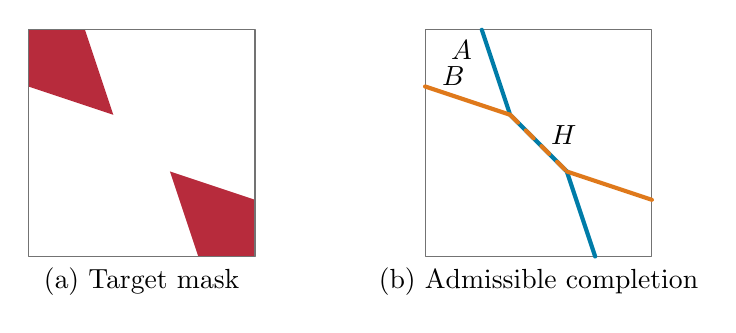
\begin{tikzpicture}[scale=.72,line cap=round,line join=round]
\begin{scope}
  \fill[paperred] (0,4)--(1,4)--(1.5,2.5)--(0,3)--cycle;
  \fill[paperred] (3,0)--(4,0)--(4,1)--(2.5,1.5)--cycle;
  \draw[black!55] (0,0) rectangle (4,4);
  \node at (2,-.45) {(a) Target mask};
\end{scope}
\begin{scope}[xshift=7cm]
  \draw[black!55] (0,0) rectangle (4,4);
  \draw[sheetA,line width=1.5pt] (1,4)--(1.5,2.5)--(2.5,1.5)--(3,0);
  \draw[sheetB,line width=1.5pt] (0,3)--(1.5,2.5);
  \draw[sheetB,line width=1.5pt] (2.5,1.5)--(4,1);
  \draw[sheetB,line width=1.5pt,dash pattern=on 4pt off 4pt]
    (1.5,2.5)--(2.5,1.5);
  \node[left] at (1,3.65) {$A$};
  \node[above] at (.5,2.85) {$B$};
  \node[right] at (2.05,2.15) {$H$};
  \node at (2,-.45) {(b) Admissible completion};
\end{scope}
\end{tikzpicture}
\caption{One top--bottom cut and one left--right cut share the middle segment.
Solid blue and orange segments are visible; the alternating segment belongs
to both sheets and is invisible in the mask. At each end of that segment,
two visible arms and one shared arm form a legal junction.}
\label{fig:completion}
\end{figure}

\section{Consequences and obstructions}
\begin{corollary}[Boundary counts]\label{cor:counts}
Let $t_T,t_B,t_L,t_R$ count genuine colour transitions along the four sides.
Every exact solution satisfies
\[
  |\mathcal A|=t_T=t_B,\qquad |\mathcal B|=t_L=t_R.
\]
Moreover, the XOR of the four corner colours is zero.
\end{corollary}
\begin{proof}
Only $A$-cuts can end on $T$ and $B$. Each has one distinct endpoint on each
side, and each endpoint changes the adjacent strip parity. The same argument
applies to $B$-cuts on $L$ and $R$. The colour difference between the two top
corners is $t_T\bmod 2$; the bottom difference is $t_B\bmod 2$. Equality of
these parities gives the corner assertion. It is a consequence of the count
condition, not an additional sufficient test.
\end{proof}

\begin{corollary}[Local degree]\label{cor:degree}
At an interior completion vertex, let $a,b,h$ count incident edges labelled
$A,B,H$. Then
\begin{equation}\label{eq:degree}
  a+h\in\{0,2\},\qquad b+h\in\{0,2\}.
\end{equation}
In particular, the number $d=a+b$ of visible boundary branches is even and
at most four. Six or more incident visible branches are impossible.
\end{corollary}
\begin{proof}
The two sums are the degrees in the two sheet subgraphs. Write them as
$2u,2v$ with $u,v\in\{0,1\}$. Then $d=2(u+v-h)$ is even and at most four.
\end{proof}
For $d=2$, either both visible arms belong to one sheet and $h=0$, or they
belong to different sheets and $h=1$. For $d=4$, necessarily $a=b=2$ and
$h=0$. In a uniform region ($d=0$), a hidden cut has $h=2$; it cannot simply
end there. These count incident edge germs at the point. Counting crossings
of a fixed-radius circle is not equivalent, since a legal cut may enter the
circle repeatedly.

\begin{corollary}[An absent family]\label{cor:absent}
If $t_L=t_R=0$, a mask is representable if and only if its entire visible
boundary is a disjoint family of simple $T$--$B$ arcs. In particular, a
representable mask with a completely uniform border is uniform throughout.
\end{corollary}
\begin{proof}
By Corollary~\ref{cor:counts}, $\mathcal B$ is empty. There can therefore be
no shared cut, and the visible boundary is exactly $\mathcal A$. Conversely,
such a boundary gives an admissible completion with no $B$- or $H$-edges.
If all four counts vanish, both families are empty and the renderer is constant.
\end{proof}

\begin{samepage}
\begin{example}[Passing local tests is not enough]\label{ex:stripe}
On a white square, put a red vertical stripe touching $T$ and $B$, together
with a red disk disjoint from the stripe and the boundary
(Figure~\ref{fig:obstructions}, left). Here $t_T=t_B=2$ and $t_L=t_R=0$;
every interior boundary point has two visible arms, and all corners are
white. Nevertheless the mask is impossible: Corollary~\ref{cor:absent}
excludes the disk's closed boundary. An isolated motif is not universally
forbidden; the absent second cut family is essential to this obstruction.
\end{example}
\end{samepage}

\begin{figure}[htbp]
\centering
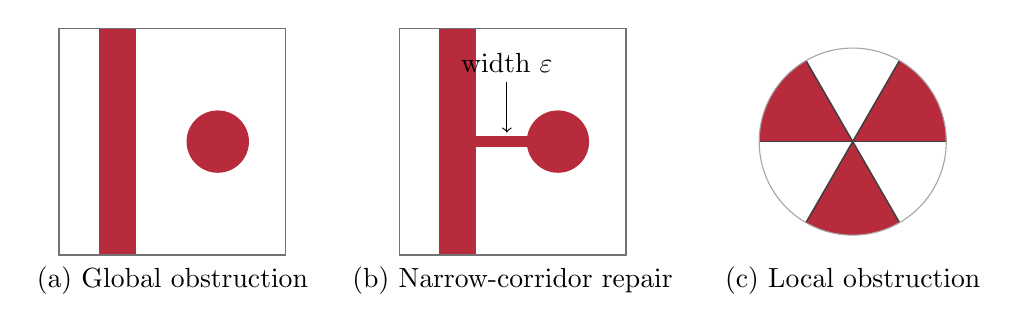
\begin{tikzpicture}[scale=.72]
\begin{scope}
  \fill[paperred] (.7,0) rectangle (1.35,4);
  \fill[paperred] (2.8,2) circle (.55);
  \draw[black!55] (0,0) rectangle (4,4);
  \node at (2,-.45) {(a) Global obstruction};
\end{scope}
\begin{scope}[xshift=6cm]
  \fill[paperred] (.7,0) rectangle (1.35,4);
  \fill[paperred] (2.8,2) circle (.55);
  \fill[paperred] (1.35,1.9) rectangle (2.8,2.1);
  \draw[black!55] (0,0) rectangle (4,4);
  \draw[thin,->] (1.9,3.05)--(1.9,2.16);
  \node[above] at (1.9,3.05) {width $\varepsilon$};
  \node at (2,-.45) {(b) Narrow-corridor repair};
\end{scope}
\begin{scope}[xshift=14cm,yshift=2cm]
  \foreach \start in {0,120,240}{
    \fill[paperred] (0,0)--(\start:1.65)
      arc[start angle=\start,end angle=\start+60,radius=1.65]--cycle;
  }
  \foreach \ang in {0,60,120,180,240,300}
    \draw[black!75,line width=.55pt] (0,0)--(\ang:1.65);
  \draw[black!35] (0,0) circle (1.65);
  \node at (0,-2.45) {(c) Local obstruction};
\end{scope}
\end{tikzpicture}
\caption{(a) Border counts and local degrees pass, but no completion exists.
(b) A thin red corridor makes the boundary two simple top--bottom arcs:
the modified mask is representable and differs by arbitrarily little area.
(c) Six branches meet at the centre, violating the degree condition;
the circle delimits the neighbourhood.}
\label{fig:obstructions}
\end{figure}

\section{Implications for reconstruction}
\paragraph{An obstruction is not an error bound.}
Keep the impossible mask in Example~\ref{ex:stripe} fixed, and join its disk
to its stripe with a red horizontal corridor of width $\varepsilon>0$
(Figure~\ref{fig:obstructions}b).
For sufficiently small $\varepsilon$, the modified boundary consists of two
simple $T$--$B$ arcs, so Corollary~\ref{cor:absent} makes it representable.
Only $O(\varepsilon)$ area is added. Thus even a fixed impossible target can
have infimum area error zero without an exact solution. A prescribed positive
paper-width constraint would obstruct this limiting construction.

\paragraph{Exact geometry, raster data and manufacture differ.}
The criterion concerns ideal two-colour regions. Blur, thresholding, cropping
or a single-pixel bridge can change the interpreted boundary graph. Applying
a proved obstruction to that graph does not certify the unknown design behind
a photograph. Likewise, a finite ordinary polynomial-cubic B\'ezier model
cannot represent every permissible smooth arc exactly: a nontrivial circular
arc already requires approximation. Minimum widths, paper-core connectivity
and cutting or threading tolerances impose further conditions beyond the
theorem. A free border changes the target and its endpoint counts; it can
remove border obstructions but need not repair interior junctions.

\paragraph{What a solver can certify.}
An embedded admissible completion certifies representability; a violated
necessary condition certifies impossibility for exact source geometry.
An infeasible restricted mixed-integer linear program only excludes its
candidate graph and constraints.
A timeout or stalled fit is inconclusive. A complete decision procedure must
exhaust all relevant connector embeddings and attachment points along visible
edges. Neither such an algorithm nor its complexity is established here.

\begin{thebibliography}{1}
\bibitem{mogensen}
Torben Mogensen.
\emph{Braided Christmas Hearts}.
7 December 2021, especially Section 4, printed pages 9--10.
\url{https://hjemmesider.diku.dk/~torbenm/hearts.pdf}.
\end{thebibliography}
\end{document}
